\newpage\backmatter
\thispagestyle{empty}
\phantomsection\addcontentsline{toc}{chapter}{外\quad{}文\quad{}资\quad{}料}
% 原文第一页,PDF缩放比例为0.95,可以自行调整
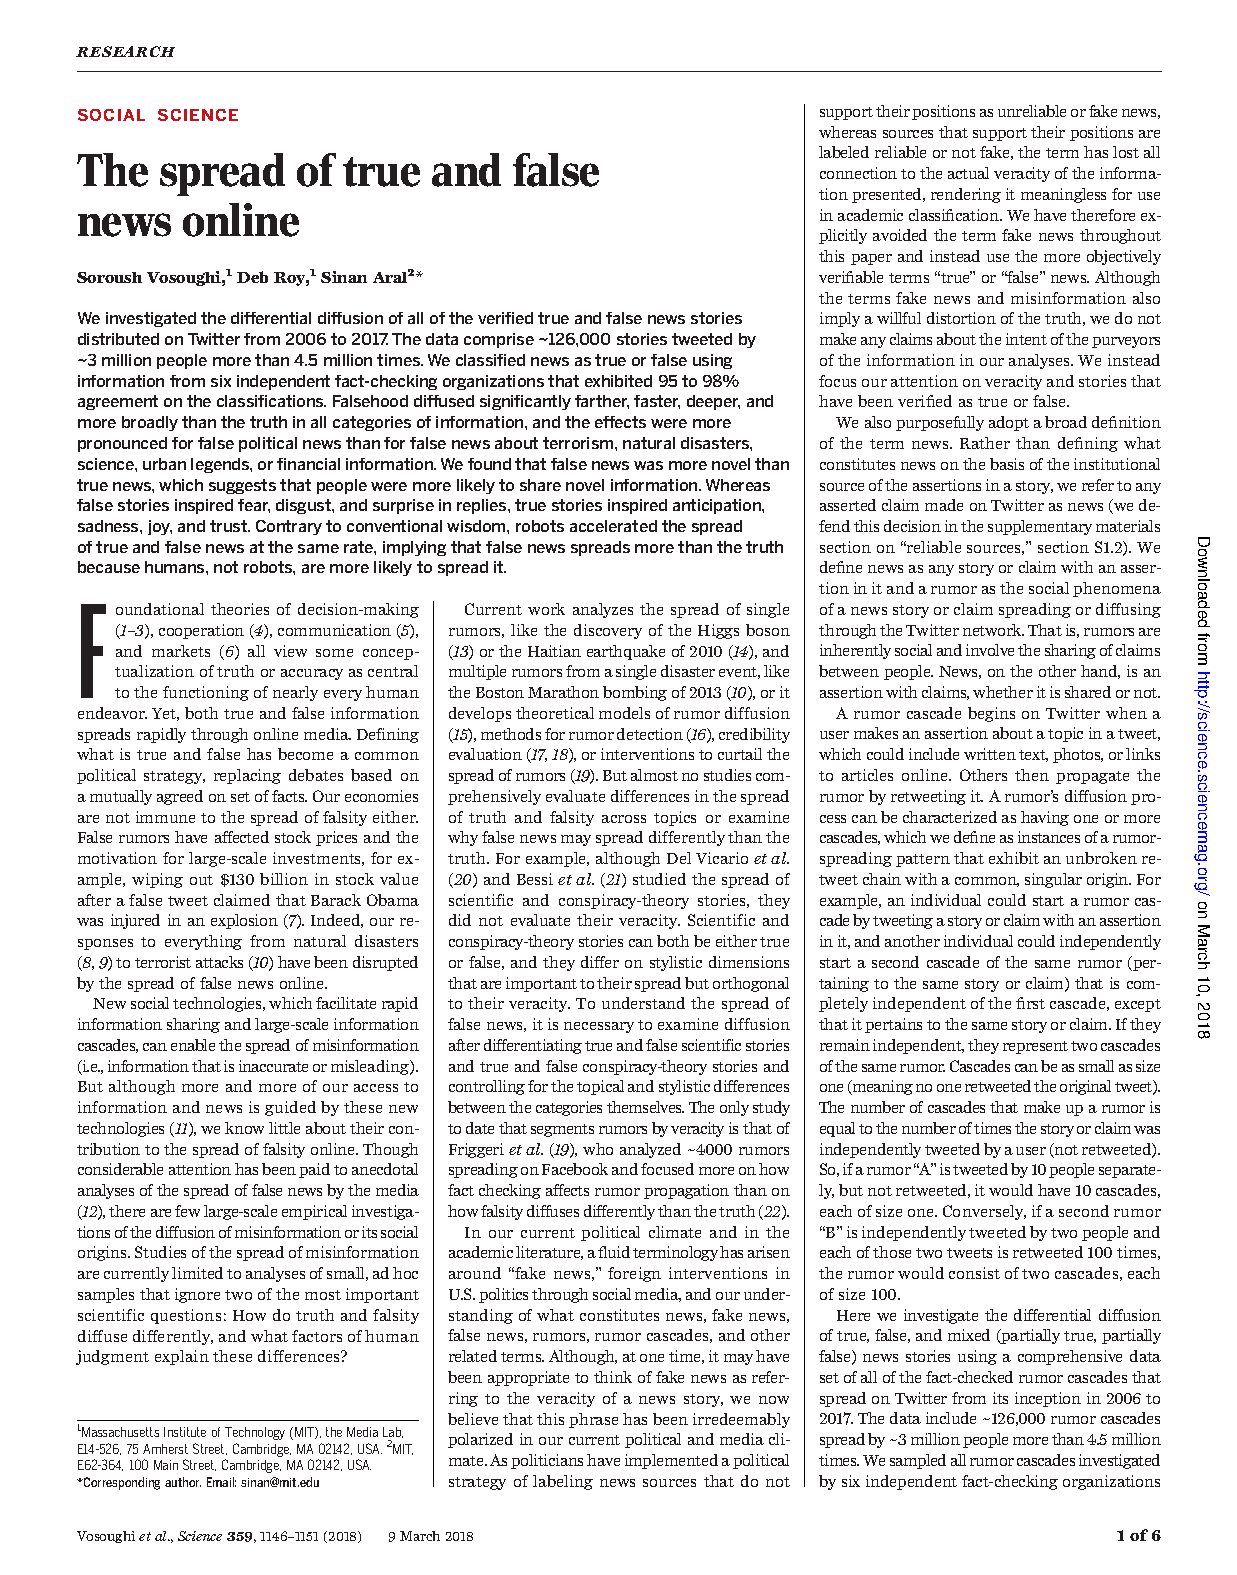
\includepdf[pages=1, scale=0.95, pagecommand=\begin{center}\translationtitlefont{外\quad{}文\quad{}资\quad{}料}\end{center}]{docs/translation.pdf}
% 原文剩余部分
\includepdf[pages=2-, scale=0.95]{docs/translation.pdf}

% Translation
\setcounter{chapter}{0}
\renewcommand{\thefigure}{~外\arabic{chapter}-\arabic{figure}~}
\renewcommand{\theequation}{~外\arabic{chapter}-\arabic{equation}~}
\renewcommand{\thetable}{~外\arabic{chapter}-\arabic{table}~}
\renewcommand{\thelstlisting}{~外\arabic{chapter}-\arabic{lstlisting}~}

\begin{center}
\phantomsection\addcontentsline{toc}{chapter}{外\quad{}文\quad{}译\quad{}文}
\translationtitlefont{外\quad{}文\quad{}译\quad{}文}
\end{center}
\vspace{8mm}
\thispagestyle{empty}


\begin{center}
\sanhao\heiti\textbf{真假新闻的在线传播}

\xiaosihao\songti{Soroush Vosoughi, Deb Roy, Sinan Aral}

\xiaosihao\songti{麻省理工学院}
\end{center}

\songti{}
\begingroup % 限制两个let语句的作用范围在外文译文部分
\let\clearpage\relax
\let\cleardoublepage\relax

%以下是排版示例,在这里为了使章节编号不出现在目录中,使用了无编号的样式,代价是这些数字都要自己书写。

\chapter*{第一章\quad{}概述}
%每一个chapter后记得以下两行
\newtranschapter

\section*{1.1\quad{}概述}
决策、合作、通信和市场领域的基础理论全都将对真实或准确度的概念化作为几乎一切人类努力的核心。然而,不论是真实信息还是虚假信息都会于在线媒体上迅速传播。定义什么是真、什么是假成了一种常见的政治策略,而不是基于一些各方同意的事实的争论。我们的经济也难免遭受虚假信息传播的影响。虚假流言会影响股价和大规模投资的动向,例如,在一条声称巴拉克·奥巴马在爆炸中受伤的推文发布后,股市市值蒸发了1300亿美元。的确,从自然灾害到恐怖袭击,我们对一切事情的反应都受到了扰乱。

新的社交网络技术在使信息的传播速度变快和规模变大的同时,也便利了不实信息(即不准确或有误导性的信息)的传播。然而,尽管我们对信息和新闻的获取越来越多地收到这些新技术的引导,但我们仍然对他们在虚假信息传播上的作用知之甚少。尽管媒体对假新闻传播的轶事分析给予了相当多的关注,但仍然几乎没有针对不实信息扩散或其发布源头的大规模实证调查。目前,虚假信息传播的研究仅仅局限于小的、局部的样本的分析上,而这些分析忽略了两个最重要的科学问题:真实信息和虚假信息的传播有什么不同?哪些人类判断中的因素可以解释这些不同?

\begin{equation}
\label{PCA_goal_appx1}
\begin{aligned}
\max_{\substack{\bm{W}}}  &  tr(\bm{W}^\mathrm{T}\bm{X}\bm{X}^ \mathrm{T}\bm{W})
\end{aligned}
\end{equation}

我只是为了把第二章挤到下一页而凑的字。我只是为了把第二章挤到下一页而凑的字。我只是为了把第二章挤到下一页而凑的字。我只是为了把第二章挤到下一页而凑的字。我只是为了把第二章挤到下一页而凑的字。我只是为了把第二章挤到下一页而凑的字。我只是为了把第二章挤到下一页而凑的字。我只是为了把第二章挤到下一页而凑的字。我只是为了把第二章挤到下一页而凑的字。我只是为了把第二章挤到下一页而凑的字。我只是为了把第二章挤到下一页而凑的字。我只是为了把第二章挤到下一页而凑的字。我只是为了把第二章挤到下一页而凑的字s。我只是为了把第二章挤到下一页而凑的字。我只是为了把第二章挤到下一页而凑的字。我只是为了把第二章挤到下一页而凑的字。我只是为了把第二章挤到下一页而凑的字。我只是为了把第二章挤到下一页而凑的字。我只是为了把第二章挤到下一页而凑的字。我只是为了把第二章挤到下一页而凑的字。我只是为了把第二章挤到下一页而凑的字。我只是为了把第二章挤到下一页而凑的字。我只是为了把第二章挤到下一页而凑的字。我只是为了把第二章挤到下一页而凑的字。

\newpage %每一章需要另起一页,为了灵活,我没有把它固定在样式中,你可以根据需求添加分页符
\chapter*{第二章\quad{}我也不知道是什么}
\newtranschapter

新的社交网络技术在使信息的传播速度变快和规模变大的同时,也便利了不实信息(即不准确或有误导性的信息)的传播。然而,尽管我们对信息和新闻的获取越来越多地收到这些新技术的引导,但我们仍然对他们在虚假信息传播上的作用知之甚少。尽管媒体对假新闻传播的轶事分析给予了相当多的关注,但仍然几乎没有针对不实信息扩散或其发布源头的大规模实证调查。目前,虚假信息传播的研究仅仅局限于小的、局部的样本的分析上,而这些分析忽略了两个最重要的科学问题:真实信息和虚假信息的传播有什么不同?哪些人类判断中的因素可以解释这些不同?

新的社交网络技术在使信息的传播速度变快和规模变大的同时,也便利了不实信息(即不准确或有误导性的信息)的传播。然而,尽管我们对信息和新闻的获取越来越多地收到这些新技术的引导,但我们仍然对他们在虚假信息传播上的作用知之甚少。尽管媒体对假新闻传播的轶事分析给予了相当多的关注,但仍然几乎没有针对不实信息扩散或其发布源头的大规模实证调查。目前,虚假信息传播的研究仅仅局限于小的、局部的样本的分析上,而这些分析忽略了两个最重要的科学问题:真实信息和虚假信息的传播有什么不同?哪些人类判断中的因素可以解释这些不同?

新的社交网络技术在使信息的传播速度变快和规模变大的同时,也便利了不实信息(即不准确或有误导性的信息)的传播。然而,尽管我们对信息和新闻的获取越来越多地收到这些新技术的引导,但我们仍然对他们在虚假信息传播上的作用知之甚少。尽管媒体对假新闻传播的轶事分析给予了相当多的关注,但仍然几乎没有针对不实信息扩散或其发布源头的大规模实证调查。目前,虚假信息传播的研究仅仅局限于小的、局部的样本的分析上,而这些分析忽略了两个最重要的科学问题:真实信息和虚假信息的传播有什么不同?哪些人类判断中的因素可以解释这些不同?

\begin{equation}
\label{PCA_goal_appx2}
\begin{aligned}
\max_{\substack{\bm{W}}}  &  tr(\bm{W}^\mathrm{T}\bm{X}\bm{X}^ \mathrm{T}\bm{W})
\end{aligned}
\end{equation}

新的社交网络技术在使信息的传播速度变快和规模变大的同时,也便利了不实信息(即不准确或有误导性的信息)的传播。然而,尽管我们对信息和新闻的获取越来越多地收到这些新技术的引导,但我们仍然对他们在虚假信息传播上的作用知之甚少。尽管媒体对假新闻传播的轶事分析给予了相当多的关注,但仍然几乎没有针对不实信息扩散或其发布源头的大规模实证调查。目前,虚假信息传播的研究仅仅局限于小的、局部的样本的分析上,而这些分析忽略了两个最重要的科学问题:真实信息和虚假信息的传播有什么不同?哪些人类判断中的因素可以解释这些不同?

新的社交网络技术在使信息的传播速度变快和规模变大的同时,也便利了不实信息(即不准确或有误导性的信息)的传播。然而,尽管我们对信息和新闻的获取越来越多地收到这些新技术的引导,但我们仍然对他们在虚假信息传播上的作用知之甚少。尽管媒体对假新闻传播的轶事分析给予了相当多的关注,但仍然几乎没有针对不实信息扩散或其发布源头的大规模实证调查。目前,虚假信息传播的研究仅仅局限于小的、局部的样本的分析上,而这些分析忽略了两个最重要的科学问题:真实信息和虚假信息的传播有什么不同?哪些人类判断中的因素可以解释这些不同?

新的社交网络技术在使信息的传播速度变快和规模变大的同时,也便利了不实信息(即不准确或有误导性的信息)的传播。然而,尽管我们对信息和新闻的获取越来越多地收到这些新技术的引导,但我们仍然对他们在虚假信息传播上的作用知之甚少。尽管媒体对假新闻传播的轶事分析给予了相当多的关注,但仍然几乎没有针对不实信息扩散或其发布源头的大规模实证调查。目前,虚假信息传播的研究仅仅局限于小的、局部的样本的分析上,而这些分析忽略了两个最重要的科学问题:真实信息和虚假信息的传播有什么不同?哪些人类判断中的因素可以解释这些不同?

\endgroup